\documentclass[fleqn,10pt]{wlscirep}
\usepackage[utf8]{inputenc}
\ifdefined\DeclareUnicodeCharacter\DeclareUnicodeCharacter{2009}{\,}\fi
\usepackage[T1]{fontenc}
\usepackage{verbatim}
%\usepackage{pdflscape}
%\usepackage{multirow}
\usepackage{booktabs}
\usepackage{multirow}
\usepackage{graphicx}
\usepackage{booktabs}
\usepackage{pdflscape}
\usepackage{tabularx}
%\usepackage{longtable}
%\usepackage{threeparttable}
\usepackage{soul}
\usepackage{lineno}
%\linenumbers
%\usepackage[nomarkers, figuresonly]{endfloat}

\title{%
    Supplementary Information for article "Stress testing insurance market stability under climate risk"
}

\author[1,*]{Simona Meiler}
\author[2]{Steven I. Jackson}
\author[3]{Kerry Emanuel}
\author[4]{Noah S. Diffenbaugh}
\author[1]{Jack W. Baker}

\affil[1]{Civil and Environmental Engineering, Stanford University, CA, USA}
\affil[2]{American Academy of Actuaries, Washington, DC, USA}
\affil[3]{Lorenz Center, Massachusetts Institute of Technology, Cambridge, Massachusetts, USA}
\affil[4]{Earth System Science, Stanford University, CA, USA}
\affil[*]{Corresponding author simona@simonameiler.ch}

\newcommand{\SITabI}{table S1}
\newcommand{\SITabII}{table S2}
\newcommand{\SITabIII}{table S3}
\newcommand{\SITabIV}{table S4}
\newcommand{\SITabV}{table S5}
\newcommand{\SITabVI}{table S6}
% \SITabVII (formerly "table S7", the variance-decomposition table) is
% retired: that table is removed from this revision (see the correction
% register, "Table S7 removal"). Tables formerly S8 and S9 are renumbered S7
% and S8 by the automatic \thetable counter below; only the literal
% cross-references in the prose (main/methods.tex, si/supporting_methods.tex)
% needed manual updates.
\newcommand{\SIFigI}{Figure~S1}
\newcommand{\SIFigII}{Figure~S2}
\newcommand{\SIFigIII}{Figure~S3}
\newcommand{\SIMethodsI}{Supplementary Methods}

\begin{document}

\flushbottom
\maketitle
\thispagestyle{empty}

\setcounter{section}{0}
\renewcommand{\thesection}{S\arabic{section}}
\renewcommand{\thefigure}{S\arabic{figure}}
\captionsetup[figure]{labelformat=default, labelsep=period, name={Fig.}}
\setcounter{figure}{0}
\renewcommand{\thetable}{S\arabic{table}}
\captionsetup[table]{labelformat=default, labelsep=period, name={Table}}
\setcounter{table}{0}

\renewcommand{\theequation}{S\arabic{equation}}
\setcounter{equation}{0}
\vspace*{1cm}

% Supporting methods relocated and rewritten from the CommsEE submission.
% Editorial comments identify scientific details that require author verification.

\section*{Text S1 Data provenance}\label{TextS1}
\subsection*{Insurance exposure and coverage}\label{DataInsuranceMarket}
We assemble the insurance market inputs from statutory filings, regulatory reports, and administrative datasets. The financial inputs describe conditions in 2024. County totals provide the link between the gridded economic loss estimates and the insurance portfolios, while insurer and statewide inputs determine capital and institutional capacity. Table~S7 summarizes the available data and the assumptions needed to connect them. Table~S8 lists the principal parameters and their treatment in the simulations.

For the private admitted market, county total insured value (TIV) comes from the Florida Hurricane Catastrophe Fund (FHCF) 2024 annual exposure report \cite{fhcf_coverage_2024}. We allocate this residential wind exposure among the top 100 individual insurers according to their statewide residential direct premiums written in 2024. The premium data come from National Association of Insurance Commissioners (NAIC) annual statements accessed through S\&P Capital IQ and Florida Office of Insurance Regulation (FLOIR) market share reports \cite{floir_marketshare_2024}. Each insurer therefore has the same relative share of the private market in every county. This assumption preserves the observed statewide market shares but does not represent geographic specialization among insurers. Insurer exposure by county is not publicly available. Its protection as a trade secret was upheld in Office of Insurance Regulation v. State Farm Florida Insurance Co. \cite{statefarm_oir_2017}.

Citizens Property Insurance Corporation, hereafter Citizens, publishes county exposure directly. We use its policies in force and exposure as of September 30, 2024, including multiperil homeowners and residential wind-only policies \cite{citizens_policies_in_force_2024}.

National Flood Insurance Program (NFIP) coverage in force and written premiums come from FEMA OpenFEMA data for policy year 2024 \cite{fema_nfip_redacted_policies_v2_2024}. County participation rates use FEMA estimates of insured residential structures relative to all residential structures within and outside Special Flood Hazard Areas (SFHAs) \cite{fema_nfip_penetration_2025}. We apply these rates to the county flood losses as described in Text~S3. Private flood insurance is not represented.
% RESOLVED S1-NFIP. Dataset snapshot confirmed: fl_risk_model/data/NfipResidentialPenetrationRates.csv, FEMA OpenFEMA "NfipResidentialPenetrationRates" dataset, asOfDate 2025-05-15, filtered to Florida's 68 counties. The baseline structure-weighted rate reproduces the reported all-county rate exactly wherever no missing-data cleaning occurred (fl_risk_model/tests/earths_future/test_nfip_allocation.py).

\subsection*{Capital and risk transfer}
Private insurer capital is statutory surplus as regards policyholders for calendar year 2024, obtained from NAIC statutory financial statements through S\&P Capital IQ. We record both entity and group surplus to represent the intragroup support described in Text~S4. Citizens' surplus comes from its 2024 annual statutory financial statement \cite{citizens_annual_statement_2024}. The NFIP fund pool is the combined National Flood Insurance Fund and Reserve Fund balance of USD~3.441~billion as of October 28, 2024 \cite{crs_nfip_fund_balance_2025}. Florida written premiums provide the denominator for the NFIP stress indicator.

FHCF inputs follow the 2023--2024 reimbursement contract. Company coverage elections of 45\%, 75\%, or 90\%, reimbursement premiums, and NAIC identifiers come from FHCF coverage selections and premium calculation reports \cite{fhcf_coverage_2024}. Retention and payout multiples follow the FHCF annual report \cite{fhcf_annual_report_2023}. We impose a statewide seasonal reimbursement cap of USD~17~billion. The model includes FHCF recoveries and catastrophe bonds but does not represent other private reinsurance treaties.

We identify outstanding catastrophe bonds covering Florida wind exposure during the 2024 hurricane season in the Artemis deal directory \cite{artemis_catbond_2024} and check their terms against sponsor offering documents and transaction disclosures. The inputs include sponsor, peril, trigger type, attachment, exhaustion, and limit. We represent indemnity, industry loss, and parametric triggers as applicable to each bond. Each bond provides a single occurrence layer within a season, without reinstatement. Text~S4 gives the payout calculation.
% PARTIALLY RESOLVED S1-BONDS. The production source file
% (fl_risk_model/data/catbonds_2024.csv) exists and was located; a
% formatted public inventory table with source dates for the data release
% was not produced in this pass (remaining work).

\section*{Text S2 Hurricane hazards and economic loss generation}\label{TextS2}
\subsection*{Historical and synthetic tracks}\label{DataTCtracks}
Historical tropical cyclone (TC) tracks come from the International Best Track Archive for Climate Stewardship (IBTrACS) \cite{knapp_international_2010}. Synthetic tracks are generated with the statistical-dynamical MIT TC model \cite{emanuel_statistical_2006,emanuel_hurricanes_2008}. We use environmental fields from ERA5 for present-day conditions \cite{hersbach_era5_2020} and five CMIP6 global climate models (GCMs) for the climate comparisons. These are CanESM5 \cite{swart_canadian_2019}, CNRM-CM6-1 \cite{voldoire_evaluation_2019}, EC-Earth3 \cite{ec-earth-consortium_2019}, IPSL-CM6A-LR \cite{hourdin_lmdz6a_2020}, and MIROC6 \cite{tatebe_description_2019}.

The ERA5 reference covers 1980--2023. Each GCM provides a historical reference for 1995--2014 and future conditions for 2041--2060 and 2081--2100 under SSP2-4.5 and SSP5-8.5. The model generates 200 TCs per year through genesis, track, and intensity simulations. This yields \num{8800} TCs in the ERA5 set and \num{4000} in each GCM, period, and scenario set before spatial filtering. We retain tracks passing within \SI{150}{\kilo\meter} of the Florida coast.

Annual frequency is derived from the fraction of seeded disturbances that develop into storms with winds above \SI{40}{\knot} under the environmental conditions of each simulation. A frequency correction adjusts the number of developed storms relative to the seeded ensemble to match the calibrated climatological baseline. The resulting frequencies retain differences among the climate simulations and are used to sample the synthetic seasons in Text~S5.
% AUTHOR CHECK S2-FREQUENCY. The calibration target, correction factor, and annual count distribution are not given in the supplied sources. Add exact settings from the hazard-generation workflow.

\subsection*{Wind fields, exposure, and vulnerability}\label{MethodsHazModel}
We calculate economic losses with CLIMADA \cite{aznar-siguan_climada_2019}, combining hazard, exposure, and vulnerability within the IPCC risk framework \cite{ipcc_managing_2012}. The Holland wind model \cite{holland_revised_2008} converts each track into a two-dimensional wind field at 120 arc-second resolution, approximately \SI{4}{\kilo\meter} at the equator. The field combines circular winds and the translational component from storm motion. Hazard intensity is the maximum lifetime 1-minute sustained wind at \SI{10}{\meter} above ground at each grid cell. Values below \SI{34}{\knot}, or \SI{17.5}{\meter\per\second}, are excluded.

The exposure layer uses LitPop \cite{eberenz_asset_2020} to disaggregate Florida's 2020 GDP by nightlight intensity and population at the same 120 arc-second resolution. These gridded values provide an economic exposure proxy. They are distinct from the residential insured values used in the financial model and do not provide property replacement costs.

We apply the USA impact function from the regional calibration of Eberenz et al. \cite{eberenz_regional_2021}. It relates wind intensity to the fraction of exposed value lost. Although wind is its hazard input, the function was calibrated against total TC economic losses and therefore incorporates the average contribution of rainfall and surge in the calibration events. We do not separately simulate rainfall or storm surge losses. Nor do we resolve differences in structural vulnerability within counties. We aggregate the gridded losses to counties before applying the financial model.

Sea-level rise is absent from the future hazard calculations. The climate experiments therefore evaluate changes represented by the synthetic TC sets while leaving this additional source of coastal flood change unmodeled.

\subsection*{Wind and flood contributions}\label{MethodsWindFloodSplit}
The insurance calculation requires separate wind and flood losses. We estimate their relative contributions with the multi-hazard regression of Gori et al. \cite{gori_sensitivity_2025,gori_tropical_2025}. That study combines county wind, precipitation, and surge intensities from physical hazard models with a damage regression calibrated to observed losses. Its synthetic TCs use the same underlying MIT track model as the present study. We use this regression to allocate our economic loss estimates between perils, rather than to calculate a second set of total losses.

For event $e$ and county $c$, the contributions in the regression are
\begin{equation}
c_{V,e,c} = \beta_V \ln V_{\text{max},e,c}, \qquad
c_{P,e,c} = \beta_P \ln\!\left(P_{\text{cum},e,c}+1\right), \qquad
c_{S,e,c} = \beta_S\, S_{\text{max},e,c},
\label{eq:hazardcontributions}
\end{equation}
where $V_{\text{max}}$, $P_{\text{cum}}$, and $S_{\text{max}}$ denote maximum wind speed, cumulative precipitation, and maximum surge. The coefficients follow the regional specification of Gori et al. \cite{gori_sensitivity_2025}. Their sum defines the compound hazard intensity
\begin{equation}
H_{e,c} = c_{V,e,c} + c_{P,e,c} + c_{S,e,c}.
\end{equation}
For each county, we select events at or above its 95th percentile of $H_{e,c}$. We then average their relative wind contributions
\begin{equation}
\tilde{r}_{V,c} =
\left\langle
\frac{c_{V,e,c}}{c_{V,e,c} + c_{P,e,c} + c_{S,e,c}}
\right\rangle_{H_{e,c}\,\geq\,H_c^{(p95)}}.
\end{equation}
Exposure weighting across Florida counties gives a statewide wind share of 84.6\%. The remaining 15.4\% comprises 10.2\% surge and 5.2\% precipitation. Figure~S2 shows the county departures from the statewide wind share. These contribution ratios are an assumption for partitioning total losses. They do not provide an event-specific reconstruction of observed damage by peril.

We sample a wind share for each event from a Beta distribution. For synthetic events, the distribution mean is 84.6\%. For the historical scenarios, the means are 70\% for Great Miami, 87.5\% for Andrew, 30\% for Lake Okeechobee, and 50\% for Irma, based on the damage reconstructions used in the model. We proportionally rescale the county shares so that their loss-weighted statewide mean equals the sampled event share. The county wind and flood losses are
\begin{equation}
L_{V,e,c}=L_{\text{total},e,c}\,r_{V,e,c}, \qquad
L_{F,e,c}=L_{\text{total},e,c}\,(1-r_{V,e,c}),
\end{equation}
where $r_{V,e,c}$ is the rescaled county share. Flood loss is the residual after wind loss. In the financial equations below, $L_{W,c}$ denotes the same wind loss as $L_{V,e,c}$, with the event index omitted.
% AUTHOR CHECK S2-SPLIT. Specify the regression coefficients and hazard units used, Beta shape parameters, sources for historical prior means, and treatment of rescaled county fractions outside [0,1]. Only the means are documented in the supplied manuscript.

\section*{Text S3 Insured loss allocation}\label{TextS3}
\subsection*{Empirical basis for the insured wind fraction}
We estimate the fraction of Florida hurricane economic losses covered by insurance using data from FLOIR, NFIP payouts, and federal disaster assistance. The reconstruction follows the approach in the U.S. Billion-Dollar Weather and Climate Disaster Database \cite{smith_us_2013,smith_quantifying_2015}. With federal assistance included, estimated economic loss is
\begin{equation}
L_{\text{econ}} = 2 \cdot L_{\text{insured}} + L_{\text{NFIP}} + L_{\text{FDA}},
\label{eq:economicreconstruction}
\end{equation}
where $L_{\text{insured}}$ is FLOIR insured loss, $L_{\text{NFIP}}$ is NFIP payouts, and $L_{\text{FDA}}$ is federal disaster assistance. The factor of two accounts for uninsured private losses in this reconstruction \cite{smith_us_2013}. Because the treatment of assistance is uncertain, we also calculate economic losses excluding $L_{\text{FDA}}$. For each estimate, the insured fraction is
\begin{equation}
f_{\text{insured}} = \frac{L_{\text{insured}}}{L_{\text{econ}}}.
\label{eq:insuredcalibration}
\end{equation}

FLOIR loss reports cover hurricane losses in 2017--2020 and 2022--2024 \cite{floir_catastrophe_2026}. NFIP payouts come from FEMA's Floodsmart database \cite{nfip_historical_2026}, and assistance from FEMA disaster summaries \cite{fema_declarations_2026}. We convert these monetary values to 2024 USD using CPI-U from the U.S. Bureau of Labor Statistics \cite{bls_cpi_2026}. Table~S1 reports both estimates for each year. The annual shares range from 11.76\% to 49.34\% across the two formulations. Mean shares for years exceeding USD~25~billion in estimated economic loss are 40.68\% with assistance included and 44.03\% with assistance excluded.

The calibration combines the annual means, the two estimation approaches, and the means for years with large losses to obtain a representative share of 38.9\%. We use a Beta$(4,6)$ distribution, with mean 0.40, for the fraction of wind loss assigned to insurance. This is an indirect calibration. The reconstructed fraction has total economic loss in its denominator, whereas the model applies it to wind loss. We therefore treat 0.40 as an allocation assumption and evaluate its influence in Text~S6. It is not a direct estimate of the proportion of properties with wind insurance.
% PARTIALLY RESOLVED S3-CALIBRATION. The median of \SITabI's six summary
% statistics (32.41, 34.24, 40.68, 38.35, 39.19, 44.03) is 38.77%, close to
% but not exactly the reported 38.9%; this is a plausible but unconfirmed
% reconstruction of the stated weighting. AUTHOR DECISION NEEDED: confirm
% the exact weighting rule, or adjust the reported figure to 38.8% (median)
% if that is in fact how it was calculated.

\subsection*{Allocation to insurance portfolios}\label{MethodsRiskAbsorption}
For county $c$, the sampled fraction $f_W$ divides economic wind loss into insured loss and a residual
\begin{equation}
L^{\mathrm{ins}}_{W,c} = f_W\, L_{W,c},
\qquad
L^{\mathrm{hh}}_{W,c} = (1-f_W)\, L_{W,c}.
\end{equation}
The residual does not enter insurer balance sheets. We allocate insured wind losses between private insurers and Citizens according to their county TIV shares. The private share is then distributed among insurers $i$
\begin{equation}
G_i = \sum_c \frac{v_{i,c}}{V^{\mathrm{priv}}_c}\,\sigma_c\, L^{\mathrm{ins}}_{W,c},
\qquad
G_{\mathrm{Cit}} = \sum_c \big(1-\sigma_c\big)\, L^{\mathrm{ins}}_{W,c},
\end{equation}
where $v_{i,c}$ is insurer $i$'s county TIV, $V^{\mathrm{priv}}_c=\sum_i v_{i,c}$, and $\sigma_c$ is the private market share of insured wind value in that county. Thus $G_i$ and $G_{\mathrm{Cit}}$ are gross insured wind losses before recoveries.

FEMA defines residential penetration as insured residential structures divided by the estimated number of residential structures, using the 2022 National Structure Inventory for the denominator \cite{fema_nfip_penetration_2025}. We use the county rate $r_{\mathrm{all},c}$, the SFHA rate $r_{\mathrm{SFHA},c}$, and the counts of all and SFHA residential structures. The SFHA fraction is $s_c=n_{\mathrm{SFHA},c}/n_{\mathrm{all},c}$, constrained to zero through one. We infer the non-SFHA rate as $(r_{\mathrm{all},c}-s_c r_{\mathrm{SFHA},c})/(1-s_c)$ and constrain it to the same range. Missing and undefined rates are set to zero. The effective county rate is $\tau_c=s_c r_{\mathrm{SFHA},c}+(1-s_c)r_{\mathrm{non},c}$. In the baseline this reproduces the county rate apart from these data cleaning steps. It weights structures, not losses within the county. The structure inventory can be incomplete, which introduces uncertainty in the denominator.

We assume this structure share also represents the fraction of flood loss insured. The county allocation is subject to aggregate coverage in force $\mathrm{CIF}_c$
\begin{equation}
L^{\mathrm{ins}}_{F,c} = \min\!\big(\tau_c\, L_{F,c},\ \mathrm{CIF}_c\big),
\qquad
L^{\mathrm{hh}}_{F,c} = L_{F,c} - L^{\mathrm{ins}}_{F,c}.
\end{equation}
All insured flood loss is assigned to the NFIP. Federal disaster assistance is used only in the empirical reconstruction above and does not enter this flood allocation.

We retain the notation $L^{\mathrm{hh}}$ and the metric name household burden for the combined uninsured wind and flood residuals in the reported results. The exposure and vulnerability inputs do not distinguish residential from nonresidential economic losses. Interpreting the entire residual as a household loss therefore depends on the model's mapping of aggregate economic losses to the residential insurance system.
% AUTHOR CHECK S3-RESIDENTIAL. Verify or add the residential mapping before describing all uninsured economic losses as household losses. No residential scaling has been invented in this revision.

\section*{Text S4 Institutional risk propagation}\label{TextS4}\label{MethodsRiskProp}
The financial calculation applies recoveries, capital, and backstop capacity to the gross losses defined in Text~S3. We apply it once to an individual event or to the combined county losses of a paired scenario or synthetic season. Each season starts from the same capital positions. The equations below specify the calculation, with the event or season index omitted for readability.

\subsection*{FHCF recoveries}
For insurer $i$, the FHCF reimbursement premium $\Pi_i$ and coverage election $p_i\in\{0.45,0.75,0.90\}$ determine retention $R_i$ and company limit $K_i$
\begin{equation}
R_i = m_{\mathrm{ret}}(p_i)\,\Pi_i,
\qquad
K_i = m_{\mathrm{pay}}\,\Pi_i.
\end{equation}
The retention multiples are $m_{\mathrm{ret}}(0.90)=6.0732$, $m_{\mathrm{ret}}(0.75)=7.2878$, and $m_{\mathrm{ret}}(0.45)=12.1464$. The payout multiple is $m_{\mathrm{pay}}=11.2368$. The recovery includes the coverage election and a loss adjustment expense factor $\lambda=1.10$
\begin{equation}
\mathrm{Rec}_i = \lambda\, p_i\, \min\!\Big(\max\big(G_i - R_i,\,0\big),\ K_i\Big).
\label{eq:fhcf}
\end{equation}
% UNRESOLVED, AUTHOR DECISION NEEDED (S4-FHCF; see correction register item
% C3). Equation retained exactly as submitted. Strong circumstantial
% evidence (the primary 2023-24 FHCF Reimbursement Contract's retention
% multiple design, confirmed to adjust the retention to 200%/120%/100% of
% its 90%-coverage base value for the 45%/75%/90% coverage elections, which
% is consistent with FHCFPremium already scaling with a company's own
% coverage election) suggests the *p_i outside the min() applies the
% election a second time to the capped portion of recovery. This was not
% changed because the exact treatment of FHCFPremium in
% fl_risk_model/data/24fin_fhcf.csv was not independently confirmed against
% the primary filing. If confirmed, recovery for companies below 90%
% coverage would increase (up to 2.22x on the capped layer at 45%
% coverage), requiring a full production rerun not possible with the
% hazard inputs available in this pass.

Total FHCF recovery cannot exceed $C_{\mathrm{FHCF}}=\$17$~billion in a season. When the aggregate uncapped recovery exceeds this amount, we reduce each recovery in proportion to its share of the total, giving $\widetilde{\mathrm{Rec}}_i=\mathrm{Rec}_i C_{\mathrm{FHCF}}/\sum_j\mathrm{Rec}_j$. Otherwise, $\widetilde{\mathrm{Rec}}_i=\mathrm{Rec}_i$. The unrecovered amount is $F_{\mathrm{FHCF}}=\max(\sum_i\mathrm{Rec}_i-C_{\mathrm{FHCF}},0)$. The loss remaining with insurer $i$ is $N_i^{\mathrm{F}}=G_i-\widetilde{\mathrm{Rec}}_i$.

\subsection*{Catastrophe bonds}
For an indemnity bond with attachment $A_i$ and limit $\mathrm{Lim}_i$, recovery is
\begin{equation}
B_i = \min\!\Big(\max\big(N^{\mathrm{F}}_i - A_i,\,0\big),\ \mathrm{Lim}_i\Big).
\end{equation}
Index and industry triggers use statewide insured wind losses before FHCF recovery. Bond payouts reduce net losses without changing FHCF recoveries. The remaining loss applied to insurer capital is $N_i=N_i^{\mathrm{F}}-B_i$.

\subsection*{Capital depletion and group support}\label{MethodsRiskTransferCapital}
We deduct net loss from statutory surplus $S_i$, leaving $E_i=S_i-N_i$. An entity with $E_i<0$ is provisionally insolvent. We then consider support within groups defined by NAIC parent identifiers. Support is available to a provisionally insolvent entity only when the ratio of group surplus to that entity's surplus exceeds 10.

For group $g$, the available pool combines surplus held outside its modeled entities and positive post-loss surplus within those entities
\begin{equation}
P_g = \max\!\Big(S^{\mathrm{grp}}_g - \textstyle\sum_{i\in g} S_i,\ 0\Big)
      \;+\; \sum_{i\in g}\max(E_i,\,0).
\end{equation}
We draw first on the parent pool and then on solvent members in proportion to their remaining surplus. Support does not push a contributing entity below zero. Eligible deficits can be covered only up to the available pool. If $C_i\geq0$ is the contribution to entity $i$, its adjusted surplus is
\begin{equation}
E'_i = E_i + C_i,
\qquad
\text{entity $i$ defaults if } E'_i < 0.
\end{equation}
This support rule is a model assumption rather than an observed commitment by the parent company.

\subsection*{FIGA assessments}
The Florida Insurance Guaranty Association (FIGA) receives the aggregate deficit of defaulted private insurers, $D_{\mathrm{FIGA}}=\sum_{i:E'_i<0}(-E'_i)$. We represent assessment capacity as 2\% normal plus 4\% emergency assessments on surviving insurers' written premiums $\Pi_{\mathrm{surv}}$. The residual is
\begin{equation}
F_{\mathrm{FIGA}} = \max\!\big(D_{\mathrm{FIGA}} - 0.06\,\Pi_{\mathrm{surv}},\ 0\big).
\end{equation}
These assessments supply one modeled funding capacity. The calculation does not simulate collections or financing over subsequent years.
% AUTHOR CHECK S4-ASSESSMENTS. Confirm the premium base, emergency assessment authority, collection horizon, and treatment of assessment-induced capital effects against code and governing terms. No legal interpretation was added during editing.

\subsection*{Citizens assessments}
Citizens' gross wind loss passes through the same modeled risk transfer steps, leaving net loss $N_{\mathrm{Cit}}$. Its deficit after surplus is $D_{\mathrm{Cit}}=\max(N_{\mathrm{Cit}}-S_{\mathrm{Cit}},0)$. We then apply two assessment tiers. The first is limited to 15\% of Citizens' premium base $\Pi_{\mathrm{Cit}}$, and the second to 10\% of the statewide property premium base $\Pi_{\mathrm{state}}$
\begin{align}
T_1 &= \min\!\big(D_{\mathrm{Cit}},\ 0.15\,\Pi_{\mathrm{Cit}}\big), \\
T_2 &= \min\!\big(D_{\mathrm{Cit}} - T_1,\ 0.10\,\Pi_{\mathrm{state}}\big), \\
F_{\mathrm{Cit}} &= \max\!\big(D_{\mathrm{Cit}} - T_1 - T_2,\ 0\big).
\end{align}
The residual $F_{\mathrm{Cit}}$ is the deficit after both modeled assessment tiers.

\subsection*{NFIP financing}
NFIP payouts first draw on the national fund pool $P_{\mathrm{NFIP}}=\$3.441$~billion. The modeled requirement beyond this pool is
\begin{equation}
\mathrm{NFIP}_{\mathrm{borrow}} = \max\!\Big(\textstyle\sum_c L^{\mathrm{ins}}_{F,c} - P_{\mathrm{NFIP}},\ 0\Big).
\end{equation}
We report this quantity as NFIP Treasury borrowing. The model applies the national fund balance to Florida claims without competing claims from other states. It does not include NFIP reinsurance or a limit on additional Treasury borrowing. The result describes a financing requirement under these assumptions, rather than borrowing necessarily available under current authority.

\subsection*{Aggregate public burden}
The submitted model defined total public burden as the sum of all four components,
\begin{equation}
B_{\mathrm{public}}^{\mathrm{legacy}} = F_{\mathrm{FHCF}} + F_{\mathrm{FIGA}} + F_{\mathrm{Cit}} + \mathrm{NFIP}_{\mathrm{borrow}}.
\label{eq:publicburdenlegacy}
\end{equation}
% RESOLVED S4-ACCOUNTING (correction register item C1). Tracing
% fl_risk_model.runner shows that capital depletion is applied to
% NetWindUSD (gross wind loss minus FHCF and cat-bond recovery), so whenever
% an insurer's or Citizens' unrecovered FHCF shortfall is not absorbed by
% its own remaining capital, it already appears inside $F_{\mathrm{FIGA}}$
% or $F_{\mathrm{Cit}}$; confirmed with deterministic fixtures
% (fl_risk_model/tests/earths_future/test_accounting_fixtures.py). Equation
% \eqref{eq:publicburdenlegacy} therefore double-counts that portion. The
% portion of the shortfall that *is* absorbed by remaining capital never
% appears in $F_{\mathrm{FIGA}}$, $F_{\mathrm{Cit}}$, or NFIP borrowing at
% all -- it is a private capital loss, not a public or quasi-public
% obligation -- so it should not be added to the aggregate either.
We therefore report a corrected, non-overlapping aggregate that excludes the FHCF shortfall entirely,
\begin{equation}
B_{\mathrm{public}} = F_{\mathrm{FIGA}} + F_{\mathrm{Cit}} + \mathrm{NFIP}_{\mathrm{borrow}},
\label{eq:publicburden}
\end{equation}
and retain equation~\eqref{eq:publicburdenlegacy} for reconciliation with the submitted values. $F_{\mathrm{FHCF}}$ is reported separately as an upstream diagnostic of FHCF capacity stress (statewide utilization of the \$17B seasonal cap), not as a fourth additive channel. Main-text Table~\ref{TabProbRPvalues}, Fig.~\ref{FigLossPublicBurdenScaling}, and \SITabIII\ use equation~\eqref{eq:publicburden}. The components measure different forms of financial stress. FIGA and Citizens residuals are deficits beyond modeled assessment capacity, borne by surviving insurers and policyholders through assessments, not by the state. NFIP borrowing is the modeled federal financing requirement and is the one component that represents a direct fiscal outlay. Their sum is an operational stress indicator. It does not establish the final distribution of costs among claimants, policyholders, taxpayers, and other parties.

\section*{Text S5 Simulations and experiments}\label{TextS5}
\subsection*{Historical and sequential stress tests}
We apply the model to the 1926 Great Miami Hurricane, 1992 Hurricane Andrew, 1928 Lake Okeechobee Hurricane, and 2017 Hurricane Irma. We also construct three pairs of events. These are Great Miami followed by Andrew, Great Miami twice, and Irma twice. Each historical or paired scenario has 200 parameter realizations with the storm tracks held fixed. The named storms define hazard footprints applied to the study's exposure and financial inputs. They are not reconstructions of the markets or losses in the years when the storms occurred.

For paired storms, the first storm reduces exposed asset values before losses from the second are calculated. Vulnerability does not change between events. These scenarios represent exposure depletion without physical recovery or further damage from changes in building condition. We combine the resulting county losses and apply the financial calculation once to the pair. Synthetic seasons likewise sum county wind and flood losses before a single financial calculation. Capital, group support, recoveries, and institutional capacity are therefore evaluated against the aggregate seasonal loss. The model does not simulate the timing of financial recoveries between storms or market recovery across successive seasons.

\subsection*{Synthetic seasons and outcome metrics}\label{MethodsOutput}
For each hazard set, we sample events with replacement according to its annual TC frequency to construct \num{10000} synthetic seasons. Retained events include all tracks within the \SI{150}{\kilo\meter} coastal buffer, including those with small or localized county losses, so a season can retain a track yet still record zero county-level loss. In the ERA5 season set, 28.5\% of seasons have zero total loss, 15.3\% have nonzero loss from exactly one contributing event, and 56.2\% have nonzero loss from two or more events.
% RESOLVED S5-COUNTS. Reproduced exactly from the archived ERA5 baseline
% (10,000 seasons; scripts/earths_future_revision/section8_historical_and_variance.py):
% 28.53% of seasons have total_damage_usd <= 0 ("no TC losses" means zero
% loss, not zero retained tracks -- every season has at least one nominally
% retained track within the 150 km buffer). Of the remaining 71.47%, 15.30%
% (of all 10,000) have exactly one contributing event and 56.17% have two or
% more. The three figures are P(zero loss), P(nonzero loss AND 1 event), and
% P(nonzero loss AND 2+ events); they sum to 100.00%.

Each realization samples the insured wind fraction, the event wind share, and a perturbation to county TIV with coefficient of variation 0.15. Other market inputs and institutional parameters remain fixed unless varied in an experiment. For each season we record economic losses, their initial insurance allocation, insurer defaults, the largest entity deficit, institutional capacity exceedances, and the public burden components. Table~S2 defines the outputs and thresholds. Text~S6 distinguishes the public burden calculations used for annual exceedance probabilities and return-period comparisons.

For a condition $\mathcal{B}$, annual exceedance probability is
\begin{equation}
P(\mathcal{B}) = \frac{1}{N}\sum_{j=1}^{N}\mathbf{1}\!\left[\mathcal{B}_j\right],
\end{equation}
where $N=\num{10000}$ and $\mathbf{1}$ indicates whether season $j$ meets the condition. The indicators include more than ten private defaults, an entity deficit above USD~1~billion, institutional capacity exceedances, NFIP claims above twice Florida NFIP annual premiums, and public burden above 1\% or 10\% of Florida GDP. Empirical return periods are the inverse of cumulative exceedance frequencies. Seasonal return periods use the synthetic year sets. Event return periods use the annual frequencies of individual storms. Figure~S1 compares both loss curves.

\subsection*{Climate comparisons}\label{MethodsFutureClim}
SSP2-4.5 provides the primary climate comparison. Tables~S4 and S5 also report SSP5-8.5. Both pathways use the same five GCMs, historical reference, future periods, and financial model. Exposure, market shares, capital, and institutional rules remain at their study values. These experiments show how the present market configuration responds to changes in hurricane hazard. They do not forecast future insurance markets.

We estimate climate effects relative to each GCM's own 1995--2014 reference and add these changes to the ERA5 baseline. This approach accounts for differences between reanalysis and GCM hazard environments when using statistical-dynamical TC simulations \cite{emanuel_hurricanes_2008,camargo_global_2013}. For each GCM, scenario, period, and metric, we subtract the historical value from the future value. We then add the median change across the five GCMs to the corresponding ERA5 value. The 10th--90th percentile range across GCM changes describes ensemble spread.

Continuous outcomes use means across \num{10000} seasons. Threshold indicators use the corresponding annual exceedance probabilities, so probability changes are added in percentage points. Text~S6 describes sampling uncertainty. No future changes in underwriting, capitalization, exposure, or regulatory policy are included.
% AUTHOR CHECK S5-DELTAS. Document the handling of negative losses or probabilities outside [0,1] after addition, and the exact combination of baseline bootstrap uncertainty with five-GCM spread. Do not imply delta correction resolves all GCM bias.

\subsection*{Market and coverage experiments}\label{MethodsPolicy}
We evaluate three prescribed interventions under present-day hazard conditions, using \num{10000} seasons for each configuration. The first two change insurance exposure and capital without changing gross wind or flood losses. The third reduces physical losses before insurance allocation.

In the private market exit experiment, Citizens' target share of insured value rises from 15\% to 25\%. Of the exposure leaving private insurers, 85\% transfers to Citizens and 15\% becomes uninsured. Private insurer surplus decreases with exposure contraction, allowing partial retention of fixed capital. Citizens' surplus scales with its market share raised to 1.3, reflecting adverse selection in exiting exposure. A change from 15\% to 25\% in share thus corresponds to a 66.7\% increase in exposure and an approximately 94\% increase in surplus. The intervention changes where losses fall and the capital available to meet them.
% PARTIALLY RESOLVED S5-EXIT. fl_risk_model/scenarios/market_exit.py
% confirms 85% of exiting exposure transfers to Citizens, 15% becomes
% uninsured, as stated. CONFIRMED DISCREPANCY: the Citizens surplus-scaling
% exponent used in the active code path
% (adjust_citizens_capital_for_growth, scaling_method="adverse_selection")
% is 1.3, not the 1.2 stated below; with the actual 15%->25% share change,
% exponent 1.3 gives a ~94% surplus increase (matching the archived
% emanuel_era5_market_exit_moderate results), not "~84%". Recommend
% correcting this paragraph's exponent and percentage to 1.3 / ~94% to
% match the code and the already-validated production results, rather than
% changing the code to match this text (see correction register).

In the coverage experiment, the target wind insured fraction rises from 40\% to 60\%, and the target flood participation rate from 11\% to 30\%. County flood changes use FEMA data within and outside SFHAs \cite{fema_nfip_penetration_2025}. The specified multipliers are 1.2 within SFHAs and 3.0 outside, applied to approximate baseline rates of 35\% and 5\%, respectively. Coastal counties receive proportional increases 1.5 times those in inland counties. NFIP policy counts, coverage, and premiums adjust proportionally. Citizens' target share falls from 15\% to 8\% as exposure transfers to private insurers and private coverage expands. Insurer surplus scales in proportion to exposure growth.
% AUTHOR CHECK S5-COVERAGE. Verify the normalization needed to reach the stated 30% flood target from the SFHA multipliers, coastal adjustment, and county weights. Keep targets distinct from measured take-up and from the wind loss allocation fraction.

In the loss reduction experiment, wind losses decrease by 30\% and flood losses by 25\% before allocation to insurance. Exposure and capital remain unchanged. This represents a prescribed effect of stronger building standards and retrofitting. The model does not simulate particular engineering measures or the costs of implementing them.

\subsection*{Loss reductions needed to offset climate effects}\label{MethodsBuildingCodeClimate}
We assess whether prescribed loss reductions can offset the mid-century SSP2-4.5 change in systemic risk. For each GCM, we simulate \num{10000} historical seasons for 1995--2014 and \num{10000} future seasons for 2041--2060. The future experiment uses 13 levels of combined wind and flood loss reduction spanning 0\% to 95\%, with wind and flood reductions applied in a fixed 3 to 2 ratio.

For each level, we subtract the GCM historical mean from the future mean after loss reduction. We add the median change across GCMs to the ERA5 baseline and report the 10th--90th percentile range. Figure~S3 shows the responses of annual total loss, private defaults, and public burden.
% AUTHOR CHECK S5-OFFSET. List all 13 reduction settings and define combined reduction and the 3 to 2 ratio precisely, including how the settings remain within physical bounds at the 95% endpoint.

\section*{Text S6 Uncertainty and evaluation procedures}\label{TextS6}
\subsection*{Estimation of public burden and return levels}
Annual public burden exceedance probabilities use the (non-overlapping, equation~\eqref{eq:publicburden}) component sum within each season. Main-text Table~\ref{TabProbRPvalues} now estimates the return level of that same season-level sum directly, rather than summing separately estimated component return levels: a sum of component quantiles generally differs from the quantile of their sum, and did so materially in the submitted version (correction register item R1). Total loss return levels remain independently ranked marginal quantiles, so Fig.~\ref{FigLossPublicBurdenScaling} compares a marginal-quantile series (total loss) with a genuine season-level-aggregate quantile series (public burden), not two marginal series.
% RESOLVED S5-QUANTILES. Recomputed as the quantile of the season-level
% aggregate (equation~\eqref{eq:publicburden}), per correction register item
% R1. The submitted component-return-level sum is retained separately in
% main-text Table~\ref{TabProbRPvalues} for reconciliation only.

\subsection*{Sampled parameters and sampling uncertainty}
The sampled parameters are the insured wind fraction, event wind share, and county TIV perturbation. The insured wind fraction follows Beta$(4,6)$. Event wind distributions have the means listed in Text~S2. County TIV has coefficient of variation 0.15. Table~S8 distinguishes these inputs from the fixed institutional parameters and the GCM ensemble.
% AUTHOR CHECK S6-DRAWS. Add the TIV distribution, dependence across counties and entities, and sampling frequency. A coefficient of variation alone does not fully specify this perturbation.

Historical scenario ranges are the 5th--95th percentiles across the 200 parameter realizations in Table~S3. For the probabilistic baseline, we bootstrap the \num{10000} ERA5 seasons \num{1000} times and report the 10th--90th percentile range. Future comparisons also report the 10th--90th percentile spread of changes across five GCMs. Parameter variation, resampling of seasons, and GCM spread describe different sources of uncertainty. They do not cover structural assumptions that remain fixed.

\subsection*{Sensitivity to the insured wind fraction}
We rerun the model at fixed wind insured fractions from 0.1 to 0.5 in steps of 0.1. Table~S6 reports mean outcomes, changes relative to 0.4, and approximate local log--log elasticities at 0.4. A value near one indicates proportional response. A value above one indicates a more than proportional response near the reference fraction.

Reducing the fraction from 0.4 to 0.1 lowers mean FIGA residual deficit by 88\% and increases uninsured wind loss by 50\%. FHCF, FIGA, and Citizens residuals have elasticities above one at the reference value. This experiment shows how allocating more wind loss to insurance affects the modeled capacity thresholds. It does not validate the allocation fraction or test the geographic distribution of insurer exposure, omitted reinsurance, or other fixed assumptions.

\subsection*{NFIP allocation sensitivity}
We test the flood-loss allocation assumption (Text~S3) with three configurations applied to the same county flood losses, wind losses, capital, seeds, and coverage caps: the baseline structure-weighted rate $\tau_c$; a limiting case that assigns county flood loss entirely within Special Flood Hazard Areas (SFHAs), using each county's SFHA participation rate; and a limiting case that assigns it entirely outside SFHAs, using each county's inferred non-SFHA rate. Configurations are restricted to zones that exist in each county (a county with no SFHA stock has no defined "SFHA-only" rate, and symmetrically for "non-SFHA-only"). These are limiting allocation scenarios, not predictions of where flood losses occur or confidence intervals: which configuration yields a higher rate varies by county (67 of 68 Florida counties have a higher SFHA rate; one does not), so neither is a uniform upper or lower bound. The baseline rate lies within the per-county envelope of the two limiting configurations for all 68 counties by construction.
% Earth's Future revision: this section replaces the removed 300-season by
% 50-parameter-draw variance decomposition (previously Table S7) as the
% Section~8 structural-sensitivity test. See the correction register,
% "Table S7 removal" and item "C6/U1," for the rationale and for what
% remains blocked (scoring these configurations against corrected insured
% flood losses and NFIP financing requires re-running the financial model
% against the same per-county, per-event flood losses used in the archived
% production run; the required cache is not distributed in this repository).

\subsection*{Consistency checks and limits of evaluation}
We compare total losses for the four historical hazard footprints with normalized losses reported by Mueller et al. \cite{muller_normalized_2025}. The estimates fall within the reported range. This provides a check on the scale of aggregate losses under the study inputs. It does not validate the county allocation, insured fraction, or financial outcomes separately.

The Irma scenario illustrates a limitation of the institutional comparison. With an assumed wind share of 50\%, the model produces low FHCF recovery, whereas the FHCF's actual Irma-related reimbursement was substantially larger, on the order of USD~6~billion, about a third of its statutory cap \cite{fhcf_annual_report_2023}. Both the modeled scenario and the historical experience remain below the fund's capacity, but agreement on capacity exhaustion does not validate the recovery amount. This difference shows why aggregate loss checks need to be distinguished from checks of allocation and institutional payments.
% RESOLVED (partially): a secondary-source figure for the Irma FHCF
% reimbursement (~USD 6B, ~36-38% of the $17B cap) is now cited. AUTHOR
% CHECK REMAINING: verify this figure and its contract year directly
% against the primary FHCF annual report (sbafla.com/media/uvmnfyka/
% 2022-fhcf-annual-report.pdf) before final submission; see correction
% register item "S6-IRMA."

The choice of hazard baseline also matters. Atlantic TC activity varies over multiple decades, so the 1980--2023 reference can differ from a longer climatology \cite{vecchi_changes_2021,emanuel_atlantic_2021,muller_normalized_2025}. Frequency choices can affect downstream losses and financial risk estimates \cite{liu_recalibrating_2026}. Figure~S1 compares event and seasonal loss curves within the chosen baseline. It does not test alternative historical baselines.

Table~S7 identifies data limitations and their possible effects. Some assumptions can affect outcomes in opposing directions. The sensitivity exercises above evaluate the parameters and structural choices varied here and do not establish an overall upper bound on systemic stress. Assessment of institutional results also requires the contractual and accounting checks noted in the main text.


\medskip
\section*{Supporting tables}
\begin{table}[htbp]
\centering
\caption{\textbf{Insured and estimated economic losses and resulting insured shares for Florida hurricane events (2017--2024)}. Economic losses are estimated using formulations including and excluding federal disaster assistance (FDA). All values are converted to 2024 USD.}
\resizebox{\textwidth}{!}{%
\label{TabInsuredFraction}
\begin{tabular}{lrrrrrr}
\hline
Year & Insured losses & Est econ loss (incl. FDA) & $f_{\text{insured}}$ (incl.) & Est econ loss (excl. FDA) & $f_{\text{insured}}$ (excl.) \\
\hline
2017 & 28,159,458,046 & 60,750,223,673 & 46.35\% & 57,644,860,280 & 48.85\% \\
2018 & 11,472,501,417 & 26,081,530,262 & 43.99\% & 23,251,364,093 & 49.34\% \\
2019 & 23,342,615     & 198,468,914     & 11.76\% & 80,793,892      & 28.89\% \\
2020 & 699,057,474    & 2,041,794,621   & 34.24\% & 1,783,712,209   & 39.19\% \\
2021 & n.a. & n.a. & n.a. & n.a. & n.a. \\
2022 & 23,914,182,689 & 56,175,193,964 & 42.57\% & 53,075,926,756 & 45.06\% \\
2023 & 318,470,377    & 1,754,055,340   & 18.16\% & 1,315,565,662   & 24.21\% \\
2024 & 7,466,073,319  & 25,060,543,556 & 29.79\% & 22,700,454,161 & 32.89\% \\
\hline
\multicolumn{2}{l}{Mean} &                & 32.41\% &                & 38.35\% \\
\multicolumn{2}{l}{Median} &              & 34.24\% &                & 39.19\% \\
\multicolumn{2}{l}{High-loss mean ($>$ \$25B)} & & 40.68\% &        & 44.03\% \\
\hline
\end{tabular}}
\end{table}
\clearpage
\begin{landscape}
\begin{table}[]
\centering
\caption{Definitions of systemic risk metrics used in the main text and Supplementary Information. Text~S4 defines the financial components and explains the interpretation of their aggregate.}
\label{TabMetricDef}
\resizebox{\linewidth}{!}{%
\begin{tabular}{@{}lll@{}}
\toprule
\textbf{Metric} &
  \textbf{Unit} &
  \textbf{Definition} \\ \midrule
\multicolumn{3}{l}{\textit{Loss decomposition}} \\
Total loss &
  USD &
  Aggregate economic tropical cyclone loss before redistribution across insurance and public backstop layers. \\
Insured wind, private &
  USD &
  Wind-related losses allocated to private admitted-market insurers in the initial risk-absorption layer. \\
Citizens wind &
  USD &
  Wind-related losses allocated to Citizens in the initial risk-absorption layer. \\
Insured flood, NFIP &
  USD &
  Flood-related losses allocated to the NFIP. \\
Un/underinsured wind &
  USD &
  Wind-related damages not covered by private insurance or Citizens because of un- or underinsurance. \\
Un/underinsured flood &
  USD &
  Flood-related damages not covered by the NFIP because of un- or underinsurance. \\
Household burden &
  USD &
  Combined uninsured wind and flood residuals under the residential mapping described in Text~S3. \\
Insured / uninsured share &
  \% &
  Share of total loss that is insured or un/underinsured. \\
\multicolumn{3}{l}{\textit{Institutional stress and public burden}} \\
FHCF shortfall &
  USD &
  Unrecovered wind losses resulting when the FHCF season-wide payout cap binds. \\
FIGA residual &
  USD &
  Residual deficit remaining after insurer insolvencies are absorbed through the FIGA, subject to its assessment limits. \\
Citizens deficit &
  USD &
  Residual deficit remaining after Citizens' surplus and assessment capacity are exhausted. \\
NFIP Treasury borrowing &
  USD &
  Florida NFIP loss above the modeled national fund pool, recorded as a Treasury financing requirement without a borrowing limit or NFIP reinsurance. \\
Total public burden &
  USD &
  Operational sum of FHCF shortfall, FIGA residual, Citizens deficit, and modeled NFIP borrowing. See Text~S4 for accounting limitations. \\
\multicolumn{3}{l}{\textit{Capital depletion and default outcomes}} \\
Private defaults &
  \# &
  Number of private insurer entities that become insolvent under a simulated event or season after modeled capital depletion. \\
Largest single-entity deficit &
  USD &
  Maximum capital shortfall of any one insurer entity in a simulated event or season. \\
\multicolumn{3}{l}{\textit{Stress ratios}} \\
FHCF utilization factor &
  ratio &
  Share of the FHCF season-wide statutory payout capacity utilized in a given scenario or simulation. A value of 1 indicates that the cap is fully used. \\
Citizens assessment stress factor &
  ratio &
  Citizens' deficit divided by its maximum assessment capacity (Tier 1 + Tier 2). Values above 1 indicate that the funding need exceeds statutory capacity. \\
FIGA stress factor &
  ratio &
  Insolvency-related deficit relative to FIGA's effective maximum assessment capacity. Values above 1 indicate exceedance of capacity. \\
NFIP Florida stress factor &
  ratio &
  Florida-attributable NFIP claims paid divided by Florida NFIP annual premium volume. \\
\multicolumn{3}{l}{\textit{Probabilistic exceedance metrics}} \\
Defaults $> 10$ &
  annual probability (\%) &
  Probability that more than ten private insurers default in a simulated tropical cyclone season. \\
Single deficit $> \$1$B &
  annual probability (\%) &
  Probability that the largest single-company deficit exceeds USD~1~billion in a simulated season. \\
FHCF $> 100\%$ cap &
  annual probability (\%) &
  Probability that modeled FHCF payouts reach or exceed the season-wide statutory cap. \\
FIGA $> 100\%$ capacity &
  annual probability (\%) &
  Probability that FIGA funding needs exceed its statutory assessment capacity. \\
Citizens $> 100\%$ capacity &
  annual probability (\%) &
  Probability that Citizens' deficit exceeds its assessment capacity. \\
NFIP $> 200\%$ annual premium &
  annual probability (\%) &
  Probability that Florida-attributable NFIP losses exceed twice Florida NFIP annual premium income. \\
Public burden $> 1\%$ Florida GDP &
  annual probability (\%) &
  Probability that total public burden exceeds 1\% of Florida's GDP in a simulated season. \\
Public burden $> 10\%$ Florida GDP &
  annual probability (\%) &
  Probability that total public burden exceeds 10\% of Florida's GDP in a simulated season. \\ \bottomrule
\end{tabular}%
}
\end{table}
\end{landscape}

\begin{landscape}
\begin{table}[htb!]
\centering
\caption{\textbf{Scenario-based loss decomposition and institutional stress outcomes for Florida hurricane events.}
Results are reported as mean values across stochastic realizations, with uncertainty ranges in parentheses indicating the 5th--95th percentiles. Metric definitions are provided in \SITabII. Named storms denote stylized hazard footprints evaluated on 2024 exposure and insurance-market conditions, not reconstructions of the original events or their realized losses.}
\label{TabScenarioStressTest}
\resizebox{\columnwidth}{!}{%
\begin{tabular}{@{}llllllll@{}}
\toprule
\textbf{Metric} &
  \textbf{Great Miami} &
  \textbf{Andrew} &
  \textbf{Lake Okeechobee} &
  \textbf{Irma} &
  \textbf{Great Miami then Andrew} &
  \textbf{Double Great Miami} &
  \textbf{Double Irma} \\ \midrule
\multicolumn{8}{l}{\textit{Loss decomposition}} \\
Total loss (USD) &
  170.4B (170.4-170.4B) &
  114.2B (114.2-114.2B) &
  156.9B (156.9-156.9B) &
  32.0B (32.0-32.0B) &
  266.5B (266.5-266.5B) &
  321.1B (321.1-321.1B) &
  62.4B (62.4-62.4B) \\
Insured wind, private (USD) &
  36.9B (20.2-56.1B) &
  29.0B (14.0-46.4B) &
  16.3B (4.3-31.6B) &
  6.0B (2.8-9.5B) &
  61.4B (35.6-90.6B) &
  69.3B (42.7-98.1B) &
  11.5B (7.4-15.9B) \\
Citizens wind (USD) &
  10.3B (4.9-17.1B) &
  10.3B (4.6-17.7B) &
  2.6B (0.7-5.1B) &
  0.5B (0.2-0.7B) &
  18.8B (9.7-30.0B) &
  19.4B (10.5-30.5B) &
  0.9B (0.6-1.2B) \\
Insured flood, NFIP (USD) &
  15.0B (4.9-27.7B) &
  4.9B (0.5-12.9B) &
  17.0B (10.5-22.4B) &
  2.6B (1.3-4.0B) &
  19.8B (9.4-31.9B) &
  28.1B (16.1-41.4B) &
  5.2B (3.6-6.7B) \\
Un/Underinsured wind (USD) &
  72.2B (42.5-101.3B) &
  60.5B (37.8-84.5B) &
  28.3B (7.6-55.4B) &
  9.7B (4.7-14.9B) &
  122.9B (84.4-165.0B) &
  136.7B (96.0-180.5B) &
  18.7B (12.8-25.5B) \\
Un/Underinsured flood (USD) &
  35.9B (11.4-66.8B) &
  9.4B (0.9-24.7B) &
  92.6B (57.3-121.9B) &
  13.3B (6.5-20.1B) &
  43.7B (20.5-70.7B) &
  67.7B (38.5-100.1B) &
  26.1B (18.0-33.8B) \\
\midrule
\multicolumn{8}{l}{\textit{Institutional stress}} \\
Total public burden (USD), corrected non-overlapping definition &
  24.4B (15.2-33.4B) &
  11.7B (4.1-22.3B) &
  18.4B (16.6-20.9B) &
  0.2B (0.0-0.8B) &
  45.4B (26.8-65.5B) &
  57.4B (39.4-76.1B) &
  3.1B (2.1-4.0B) \\
% CORRECTED (register item C1): excludes FHCF shortfall from the sum
% (FIGA + Citizens + NFIP only); submitted values were 26.1 / 11.7 / 18.4 /
% 0.2 / 51.0 / 65.4 / 3.1. Unchanged for scenarios with zero FHCF shortfall
% in this run (Andrew, Lake Okeechobee, Irma, Double Irma).
FHCF shortfall (USD), diagnostic only, not summed above &
  1.7B (0.0-8.0B) &
  0.0B (0.0-0.0B) &
  0.0B (0.0-0.0B) &
  0.0B (0.0-0.0B) &
  5.6B (0.0-11.6B) &
  8.0B (0.0-12.7B) &
  0.0B (0.0-0.0B) \\
FIGA residual (USD) &
  7.0B (3.2-13.4B) &
  4.2B (1.1-10.0B) &
  3.3B (0.0-8.8B) &
  0.1B (0.0-0.7B) &
  15.8B (6.2-27.7B) &
  19.1B (8.5-31.1B) &
  1.3B (0.1-2.8B) \\
Citizens deficit (USD) &
  5.8B (3.1-11.4B) &
  5.2B (1.9-11.9B) &
  1.6B (0.0-4.0B) &
  0.0B (0.0-0.0B) &
  13.2B (4.7-24.1B) &
  13.6B (5.5-24.7B) &
  0.0B (0.0-0.3B) \\
NFIP treasury borrowing (USD) &
  11.5B (1.4-24.3B) &
  2.2B (0.0-9.4B) &
  13.6B (7.1-18.9B) &
  0.1B (0.0-0.5B) &
  16.4B (6.0-28.5B) &
  24.7B (12.7-38.0B) &
  1.8B (0.2-3.3B) \\
\hline
\textit{Capital \& default assessment} & & & & & & & \\
Private defaults (\#) &
  18 (15-22) &
  16 (12-20) &
  13 (0-18) &
  5 (0-11) &
  21 (18-23) &
  22 (19-24) &
  12 (8-14) \\
Largest single-entity deficit (USD) &
  1.9B (1.1-3.3B) &
  1.2B (0.4-2.8B) &
  1.0B (0.0-2.4B) &
  0.1B (0.0-0.4B) &
  3.8B (1.6-6.8B) &
  4.6B (2.2-7.5B) &
  0.6B (0.2-1.0B) \\
\midrule
\multicolumn{8}{l}{\textit{Stress ratios}} \\
FHCF utilization factor &
  0.79 (0.20-1.00) &
  0.74 (0.25-0.93) &
  0.02 (0.00-0.08) &
  0.00 (0.00-0.00) &
  0.98 (0.87-1.00) &
  0.98 (0.92-1.00) &
  0.00 (0.00-0.01) \\
Citizens assessment stress factor &
  6.46 (3.43-12.64) &
  5.83 (2.16-13.26) &
  1.74 (0.00-4.46) &
  0.00 (0.00-0.00) &
  14.67 (5.26-26.77) &
  15.13 (6.07-27.40) &
  0.06 (0.00-0.29) \\
FIGA stress factor &
  0.95 (0.91-0.98) &
  0.88 (0.74-0.97) &
  0.77 (0.00-0.97) &
  0.17 (0.00-0.67) &
  0.98 (0.95-0.99) &
  0.98 (0.97-0.99) &
  0.70 (0.23-0.89) \\
NFIP Florida stress factor &
  10.73 (3.49-19.86) &
  3.54 (0.35-9.23) &
  12.19 (7.56-16.02) &
  1.90 (0.95-2.85) &
  14.20 (6.74-22.89) &
  20.13 (11.54-29.68) &
  3.71 (2.58-4.79) \\
\bottomrule

\end{tabular}%
}
\end{table}
\end{landscape}

\begin{landscape}
\begin{table}[htb!]
\centering
\caption{\textbf{Loss decomposition and public institutional burden across climate and policy scenarios.}
Values show expected annual losses and institutional burdens under present-day baseline conditions, future climate scenarios (2050 and 2100 under SSP2-4.5 and SSP5-8.5), and illustrative market and policy interventions evaluated under present-day climate forcing. Values are reported as means in billion USD with uncertainty ranges (10th--90th percentile) in parentheses.}
\label{TabClimatePolicyLosses}

\small
\setlength{\tabcolsep}{4pt}

\begin{tabular}{@{}l|l|llll|lll@{}}
\toprule
\textbf{Metric (USD B)} &
\textbf{Baseline} &
\textbf{2050 SSP2-4.5} &
\textbf{2050 SSP5-8.5} &
\textbf{2100 SSP2-4.5} &
\textbf{2100 SSP5-8.5} &
\textbf{Market Exit} &
\textbf{Insurance Penetration} &
\textbf{Building Codes} \\
\midrule

\multicolumn{9}{l}{\textit{Loss decomposition}} \\
Total loss                         & 19.3 (0.0--37.8) & 31.5 (15.3--45.5) & 34.9 (17.6--55.6) & 41.9 (18.3--50.0) & 59.2 (22.2--104.2) & 19.3 (0.0--37.8) & 19.3 (0.0--37.9) & 13.7 (0.0--27.9) \\
Insured wind, private            & 5.5 (0.0--11.6) & 13.9 (6.7--19.9) & 15.4 (7.8--24.3) & 18.5 (8.1--22.1) & 26.2 (9.8--46.0) & 4.7 (0.0--9.8) & 8.1 (0.0--17.3) & 3.8 (0.0--8.1) \\
Citizens wind                      & 1.1 (0.0--1.8) & 2.6 (1.3--3.8) & 2.9 (1.5--4.6) & 3.4 (1.5--4.1) & 4.7 (1.8--8.6) & 1.9 (0.0--3.5) & 1.7 (0.0--2.8) & 0.8 (0.0--1.2) \\
Insured flood, NFIP              & 0.6 (0.0--0.9) & 1.5 (0.8--2.3) & 1.7 (0.8--2.7) & 1.9 (0.9--2.3) & 2.7 (1.0--5.0) & 0.6 (0.0--0.9) & 1.7 (0.0--2.4) & 0.5 (0.0--0.7) \\
Un/underinsured wind               & 9.7 (0.0--19.8) & 7.3 (3.6--10.8) & 8.3 (4.1--13.1) & 9.9 (4.3--11.8) & 14.0 (5.2--24.5) & 9.7 (0.0--19.8) & 6.5 (0.0--13.4) & 6.8 (0.0--13.8) \\
Un/underinsured flood              & 2.4 (0.0--3.9) & 6.2 (2.9--8.8) & 6.6 (3.4--10.8) & 8.2 (3.5--9.6) & 11.5 (4.3--20.1) & 2.4 (0.0--3.9) & 1.3 (0.0--2.0) & 1.8 (0.0--2.9) \\
% CORRECTED (register item C5): Building Codes column (last), Total loss and
% Un/underinsured wind/flood. fl_risk_model/mc_run_events.py captured
% wind_total/water_total before the building-code loss-reduction block, so
% total_damage_usd never reflected the prescribed reduction while insured
% components (computed from the correctly reduced damage) shrank -- this
% inflated the un/underinsured residual. Code fixed; values above are
% reconstructed post hoc from the still-correct component columns
% (scripts/earths_future_revision/section9_climate_policy_tables.py).
% Submitted values were 19.3 (0.0-38.0) / 11.7 (0.0-23.8) / 2.6 (0.0-4.1).

\midrule
\multicolumn{9}{l}{\textit{Institutional stress}} \\
Total public burden, corrected non-overlapping definition & 2.4 (0.0--1.9) & 7.1 (3.3--11.0) & 7.8 (4.0--13.9) & 9.6 (4.1--12.3) & 14.9 (5.1--29.7) & 2.7 (0.0--2.8) & 4.4 (0.0--3.6) & 1.5 (0.0--0.7) \\
% CORRECTED (register items C1 + C5): Baseline, Market Exit, Insurance
% Penetration, and Building Codes columns use the corrected, non-overlapping
% burden definition (FIGA + Citizens + NFIP; submitted values 2.7 / 3.1 /
% 5.1 / 1.6). AUTHOR CHECK REMAINING: the five climate-scenario columns
% (2050/2100 x SSP2-4.5/SSP5-8.5) above still use the submitted legacy
% definition and have not been recomputed under the GCM-ensemble delta
% procedure in this pass -- see correction register item C1 and
% scripts/analysis/compute_climate_deltas.py for the extension needed.
FHCF shortfall (diagnostic, not summed above) & 0.3 (0.0--0.0) & 1.0 (0.4--1.6) & 1.1 (0.6--2.1) & 1.5 (0.6--2.0) & 2.5 (0.8--5.1) & 0.4 (0.0--0.0) & 0.7 (0.0--0.0) & 0.2 (0.0--0.0) \\
FIGA residual                      & 1.3 (0.0--1.0) & 3.4 (1.6--5.2) & 3.8 (1.9--6.6) & 4.7 (2.0--6.0) & 7.3 (2.5--14.3) & 1.1 (0.0--0.7) & 2.0 (0.0--1.0) & 0.8 (0.0--0.3) \\
Citizens deficit                   & 0.7 (0.0--0.7) & 1.8 (0.9--2.8) & 2.0 (1.0--3.4) & 2.4 (1.0--3.0) & 3.5 (1.3--6.9) & 1.3 (0.0--2.1) & 1.2 (0.0--1.6) & 0.5 (0.0--0.2) \\
NFIP Treasury borrowing            & 0.3 (0.0--0.0) & 0.8 (0.4--1.4) & 0.9 (0.5--1.7) & 1.0 (0.4--1.4) & 1.7 (0.6--3.4) & 0.3 (0.0--0.0) & 1.2 (0.0--0.0) & 0.2 (0.0--0.0) \\

\bottomrule
\end{tabular}
\end{table}

%\begin{landscape}
\begin{table}[htb!]
\centering
\caption{\textbf{Probabilistic exceedance of systemic insurance stress thresholds across climate and policy scenarios.}
Annual exceedance probabilities (percent) of systemic stress thresholds for private insurers, public and quasi-public institutions, and aggregate fiscal impact, estimated from \num{10000} simulated tropical cyclone seasons. Results are shown for present-day conditions, mid-century (2050) and end-of-century (2100) climate scenarios under SSP2-4.5 and SSP5-8.5, as well as illustrative market and policy interventions evaluated under present-day climate forcing. Values denote mean probabilities, with uncertainty ranges (10th--90th percentile) in parentheses.}
\label{TabSystemicRiskProb}

\small
\setlength{\tabcolsep}{3.5pt}

\begin{tabular}{@{}l|l|llll|lll@{}}
\toprule
\textbf{Metric (\%)} &
  \textbf{Baseline} &
  \textbf{2050 SSP2-4.5} &
  \textbf{2050 SSP5-8.5} &
  \textbf{2100 SSP2-4.5} &
  \textbf{2100 SSP5-8.5} &
  \textbf{Market Exit} &
  \textbf{Insurance Penetration} &
  \textbf{Building Codes} \\ \midrule

Defaults > 10 &
  11.4 (10.9-11.8) &
  17.7 (12.6-20.6) &
  18.8 (13.1-22.2) &
  20.2 (13.5-21.3) &
  22.7 (14.6-27.3) &
  10.3 (9.9-10.7) &
  9.7 (9.3-10.0) &
  9.2 (8.8-9.6) \\

Single Deficit > \$1B &
  7.2 (6.9-7.5) &
  11.5 (7.9-14.2) &
  12.2 (8.6-15.9) &
  13.5 (8.8-15.1) &
  16.6 (9.9-22.8) &
  6.5 (6.2-6.8) &
  8.2 (7.9-8.6) &
  5.6 (5.3-5.9) \\

\midrule

FHCF > 100\% Cap &
  0.8 (0.7-0.9) &
  0.9 (0.7-1.1) &
  1.0 (0.7-1.2) &
  1.0 (0.7-1.1) &
  1.2 (0.8-1.6) &
  0.7 (0.6-0.8) &
  1.2 (1.0-1.3) &
  0.5 (0.4-0.6) \\

FIGA > 100\% Capacity &
  13.6 (13.2-14.1) &
  22.1 (15.1-27.5) &
  23.3 (16.6-30.9) &
  26.0 (17.0-29.4) &
  32.3 (19.0-45.3) &
  12.8 (12.3-13.2) &
  13.4 (13.0-13.9) &
  11.5 (11.1-11.9) \\

Citizens > 100\% Capacity &
  9.5 (9.2-9.9) &
  15.1 (10.4-18.8) &
  16.1 (11.2-20.8) &
  17.3 (11.5-19.4) &
  21.0 (12.6-29.5) &
  13.0 (12.6-13.4) &
  11.8 (11.3-12.2) &
  7.9 (7.6-8.3) \\

NFIP > 200\% Annual Premium &
  5.0 (4.8-5.3) &
  5.9 (4.4-6.9) &
  6.1 (4.6-7.5) &
  6.6 (4.7-7.2) &
  7.7 (5.0-10.0) &
  5.0 (4.8-5.3) &
  9.3 (8.9-9.7) &
  4.0 (3.7-4.2) \\

\midrule

Public Burden > 1\% FL GDP &
  3.7 (3.5-3.9) &
  4.3 (3.2-5.1) &
  4.5 (3.4-5.5) &
  4.9 (3.4-5.3) &
  5.6 (3.7-7.3) &
  4.3 (4.0-4.5) &
  5.6 (5.3-5.9) &
  2.4 (2.2-2.6) \\

Public Burden > 10\% FL GDP &
  0.1 (0.1-0.2) &
  0.2 (0.1-0.2) &
  0.2 (0.1-0.2) &
  0.2 (0.1-0.2) &
  0.2 (0.1-0.3) &
  0.2 (0.1-0.3) &
  0.7 (0.6-0.8) &
  0.0 (0.0-0.1) \\

\bottomrule
\end{tabular}
\end{table}
\end{landscape}

\begin{table}[htb!]
\centering
\small
\caption{\textbf{Sensitivity of model outputs to the insured wind loss fraction.} Mean values (in \$B; insurer defaults reported as counts) for each output metric across five fixed values of the insured wind fraction $f$. The table also reports the relative change compared to the reference case ($f = 0.4$, the mean of the baseline Beta(4,\,6) prior) and the approximate log--log elasticity $\varepsilon$ evaluated at $f = 0.4$. Metrics with $\varepsilon \approx 0$ are invariant to the insured fraction by construction; $\varepsilon = 1$ indicates proportional scaling; and $\varepsilon > 1$ indicates amplification through the insurance system.}
\label{tab:si_insured_frac}
\resizebox{\textwidth}{!}{%
\begin{tabular}{lrrrrr|rrrrr}
\toprule
& \multicolumn{5}{c|}{Mean value (\$B)} & \multicolumn{4}{c}{Change vs.\ $f{=}0.4$} & \\
\cmidrule(lr){2-6}\cmidrule(lr){7-10}
Metric & $f{=}0.1$ & $f{=}0.2$ & $f{=}0.3$ & $f{=}0.4$ & $f{=}0.5$ & $\Delta_{0.1}$ & $\Delta_{0.2}$ & $\Delta_{0.3}$ & $\Delta_{0.5}$ & $\varepsilon$ \\
\midrule
\multicolumn{11}{l}{\textit{Loss decomposition}} \\\\
Wind insured, private & 1.36 & 2.72 & 4.08 & 5.44 & 6.80 & -75\% & -50\% & -25\% & +25\% & +1.00 \\
Wind insured, Citizens & 0.27 & 0.53 & 0.80 & 1.07 & 1.34 & -75\% & -50\% & -25\% & +25\% & +1.00 \\
Wind un/underinsured & 10.26 & 9.12 & 7.98 & 6.84 & 5.70 & +50\% & +33\% & +17\% & -17\% & -0.66 \\
\addlinespace
\multicolumn{11}{l}{\textit{Institutional stress}} \\\\
FHCF shortfall & 0.02 & 0.10 & 0.22 & 0.36 & 0.50 & -95\% & -74\% & -39\% & +39\% & +1.60 \\
FIGA residual deficit & 0.15 & 0.46 & 0.84 & 1.27 & 1.72 & -88\% & -64\% & -34\% & +36\% & +1.40 \\
Citizens residual deficit & 0.12 & 0.29 & 0.49 & 0.71 & 0.94 & -84\% & -60\% & -31\% & +32\% & +1.28 \\
\addlinespace
\multicolumn{11}{l}{\textit{Capital / defaults}} \\\\
Insurer defaults (count) & 0.8186 & 1.4122 & 1.8586 & 2.1992 & 2.4831 & -63\% & -36\% & -15\% & +13\% & +0.57 \\
Largest entity deficit & 0.05 & 0.13 & 0.22 & 0.32 & 0.43 & -84\% & -59\% & -31\% & +32\% & +1.25 \\
\bottomrule
\end{tabular}}
\end{table}

\newpage
% REMOVED (Earth's Future revision, correction register: "Table S7 removal").
% The submitted variance-decomposition table (300 seasons x 50 parameter
% draws, one-way ANOVA eta^2) is removed here, along with the associated
% hazard-dominance / broad-robustness claims that cited it. The 300 seasons
% were selected to span the loss distribution rather than drawn at random,
% so the reported variance shares describe that specific design and do not,
% on their own, establish robustness to all structural assumptions or to a
% randomly sampled season -- a scope limitation the submitted text already
% partly acknowledged but that this revision treats as a reason to remove
% the table rather than qualify it further. The focused NFIP allocation test
% (Text~S3, Table~S6) and the insured-fraction sensitivity (Table~S6) are
% more directly relevant to the manuscript's central claims and are
% retained. The research code
% (scripts/run/run_variance_decomposition.py) and archived results are
% unchanged and remain available; this revision independently reproduced
% every eta^2 value reported in the submitted table exactly
% (docs/earths_future_revision/correction_register.md item "S6-ANOVA";
% results/earths_future_revision/historical/table_S7_audit_retained_for_code_reference.csv).
% Tables S8 and S9 below are renumbered to S7 and S8.

\begin{table*}[t]
\centering
\caption{\textbf{Ideal data inputs and the publicly available proxies and models used in this study.}
For each component of the modeling framework, we list the data that a regulator or supervisor with statutory data-collection authority could, in principle, obtain (ideal data input), the public proxy or model adopted here, and the implications for interpreting model outcomes. The effects listed here are not a quantitative bias assessment.}
\label{tab:data_requirements}
\footnotesize
\renewcommand{\arraystretch}{1.10}
\resizebox{0.92\textwidth}{!}{%
\begin{tabular}{@{}p{0.155\textwidth} p{0.275\textwidth} p{0.275\textwidth} p{0.205\textwidth}@{}}
\toprule
\textbf{Component} & \textbf{Ideal data inputs} & \textbf{Public proxy or model used here} & \textbf{Effect on systemic-risk estimates} \\
\midrule
\multicolumn{4}{@{}l}{\textit{Hazard and loss generation}}\\
\midrule
TC hazard & TC event catalog including wind, rainfall, and storm-surge fields and future sea-level-rise (SLR) projections & Historical (IBTrACS) and synthetic (MIT model) TC events for present and future climate; peak sustained wind as the hazard, with rainfall and surge represented indirectly (see Vulnerability and Wind--flood split) & Omits additional coastal flood change from SLR. Baseline period affects TC frequency and losses. Net effect is not quantified \\
Asset exposure & Property-level replacement-cost values (TIV) by structure and occupancy & 2020 GDP disaggregated with LitPop using nightlight intensity and population at approximately 4\,km resolution & Economic exposure proxy includes nonresidential assets. Its mapping to residential losses requires an allocation assumption (Text~S3) \\
Vulnerability & Residential, structure-specific damage functions & Regionally calibrated USA impact function, wind-parameterized, fit to total losses & Includes nonresidential damage and average rainfall and surge contributions. Does not resolve local building vulnerability \\
Wind--flood split & Event-level claims by peril (wind, surge, rainfall) & County-level multi-hazard regression (Gori et al.\ 2025); climatological mean shares & Peril allocation is approximate and shifts losses between wind insurers and the NFIP \\
\midrule
\multicolumn{4}{@{}l}{\textit{Insurance-system layers}}\\
\midrule
Private wind insurers (exposure) & Policy- or property-level premiums, coverage, and exposure by carrier and county & County TIV from FHCF allocated to carriers by statewide direct premium shares & Removes geographic specialization. The effect on simultaneous defaults and FIGA demand has not been quantified \\
Insurer capital & Full balance sheets, risk-based capital, internal models, parent guarantees, and cross-line support & Statutory surplus (entity and group) with a group-support rule & Support follows an assumed rule. Actual commitments and capital available from other business lines are not observed \\
Reinsurance (FHCF) & Per-company FHCF elections and realized recoveries & Published FHCF reimbursement-contract terms and per-company elections (retention, coverage \%, USD~17\,B seasonal cap) & Uses published terms. Recovery timing and placement of the company limit require contractual interpretation \\
Reinsurance (private treaties) & Per-carrier quota-share, excess-of-loss, retrocession, and industry-loss-warranty programs & Not represented (omitted) & Recoverable private reinsurance would reduce retained loss for covered claims. The magnitude is not estimated \\
Catastrophe bonds & Full insurance-linked-securities positions and triggers by sponsor & Public deal terms (Artemis); single-occurrence layers & Public disclosures may omit coverage or trigger details. The magnitude of omitted recovery is not estimated \\
Insured share (wind) & Observed take-up and coverage adequacy by county and peril & Billion-Dollar Disaster reconstruction ($\approx$40\% in large events); Beta(4,6) & Calibrated against total economic losses and applied to wind losses. Sensitivity is reported in Table~S6 \\
NFIP flood & Policy-level NFIP coverage and claims, plus the private-flood market & County coverage-in-force, take-up rates, Florida premium, and fund balance & Structure-based take-up is applied to economic losses. Private flood coverage and variation in loss within counties are absent \\
Citizens & Policy-in-force and claims detail & Published county exposure, statutory surplus, Tier~1/Tier~2 premium bases & Uses observed county exposure and surplus with simplified assessment capacity \\
FIGA & Realized insolvency deficits and assessable-premium base & Statutory caps (2\% normal plus 4\% emergency) on surviving-insurer premium & Represents assessment capacity using surviving premium. Does not model subsequent collections or financing \\
NFIP backstop & Fund balance, reinsurance, and Treasury borrowing authority & Modeled fund pool (USD~3.441\,B) plus Treasury borrowing & Omits NFIP reinsurance, other states' claims, and the borrowing limit. These omissions can affect financing needs in different directions \\
\bottomrule
\end{tabular}}
\end{table*}

\begin{table}[ht]
\centering
\caption{\textbf{Model parameters and uncertainty treatment in the risk-propagation framework.}
Each parameter is classified as \emph{deterministic} (held fixed across all simulations), \emph{stochastic} (resampled each Monte Carlo iteration), or \emph{uncertain} (varied across the climate-model ensemble). Data inputs and their public proxies are summarised separately in Table~S7.}
\label{tab:si-parameters}
\small
\renewcommand{\arraystretch}{1.25}
\begin{tabularx}{\textwidth}{@{}%
  >{\raggedright\arraybackslash}p{4.0cm}%
  >{\raggedright\arraybackslash}p{4.0cm}%
  >{\raggedright\arraybackslash}p{4.0cm}%
  >{\raggedright\arraybackslash}X@{}}
\toprule
Parameter & Value & Source & Treatment \\
\midrule
\multicolumn{4}{@{}l}{\textit{Stochastic (sampled each iteration)}}\\
\addlinespace[2pt]
Insured wind fraction $f_W$ & $\mathrm{Beta}(4,6)$, mean $0.40$ & Florida loss reconstruction (Text~S3) & Stochastic; swept $0.1$--$0.5$ (Table~S6) \\
Wind/flood loss share & Beta prior, mean $0.846$ (wind) & Gori et al.\ (2025), county $P_{95}$ & Stochastic; the dominant driver of variance in flood-side metrics \\
TIV perturbation & $\mathrm{CoV}=0.15$ & Assumed & Stochastic \\
\addlinespace[3pt]
\multicolumn{4}{@{}l}{\textit{Deterministic (fixed across simulations)}}\\
\addlinespace[2pt]
Number of simulated seasons $N$ & $10{,}000$ & Model configuration & Deterministic \\
FHCF seasonal cap & \$17\,B & FHCF statute / 2023--24 report & Deterministic \\
FHCF coverage election $\mathrm{cov}_i$ & $\{45,75,90\}\%$ & FHCF reimbursement contract & Deterministic; assigned by insurer \\
FHCF retention and payout-limit multiples & retention multiples $12.1464$ (45\%), $7.2878$ (75\%), $6.0732$ (90\%); payout multiple $11.2368$; expense factor $1.10$ & FHCF reimbursement contract & Deterministic \\
FIGA assessment cap & $2\%$ normal $+\,4\%$ emergency of surviving premium & Fla.\ Stat.\ \S631.57 & Deterministic \\
Citizens Tier~1 / Tier~2 caps & $15\%$ / $10\%$ of respective premium bases & Citizens enabling statute & Deterministic \\
NFIP fund pool & \$3.441\,B & CRS IN10784 & Deterministic \\
Intragroup support rule & group/entity surplus ratio $>10$; eligible deficits cured up to the available group pool & Stylized rule; surplus from S\&P filings & Deterministic \\
\addlinespace[3pt]
\multicolumn{4}{@{}l}{\textit{Uncertain (varied across the climate ensemble)}}\\
\addlinespace[2pt]
Climate-change deltas & 5-GCM ensemble median, 10th--90th percentile range & CMIP6 / MIT TC model & Uncertain (ensemble range reported) \\
\bottomrule
\end{tabularx}
\end{table}

\clearpage
\section*{Supporting figures}

\begin{figure*}[ht]
    \centering
    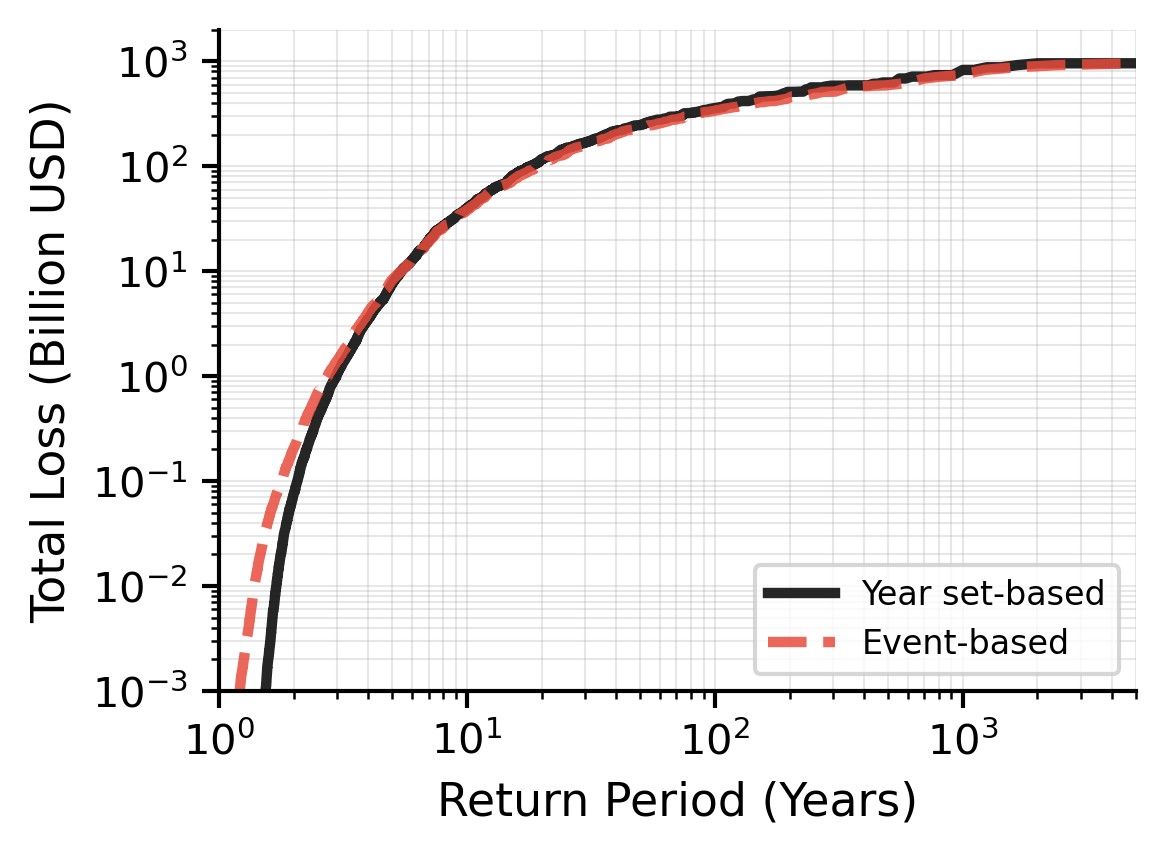
\includegraphics[width=0.45\textwidth]{figures/fig_loss_return_period.png}
    \caption{\textbf{Return period curves for total tropical cyclone losses in Florida.} 
    Event-based losses (red dashed line) and seasonal aggregate losses (solid black line) are shown. 
    Event-based return periods are derived from the empirical exceedance distribution of single events in the ERA5 synthetic tropical cyclone event set (\num{8800} events covering 1980--2023; Text~S2). Seasonal return periods are computed from the empirical exceedance distribution of aggregate losses across simulated \num{10000} tropical cyclone years (Text~S5).}
\label{FigEventRP}
\end{figure*}

\begin{figure*}[ht]
    \centering
    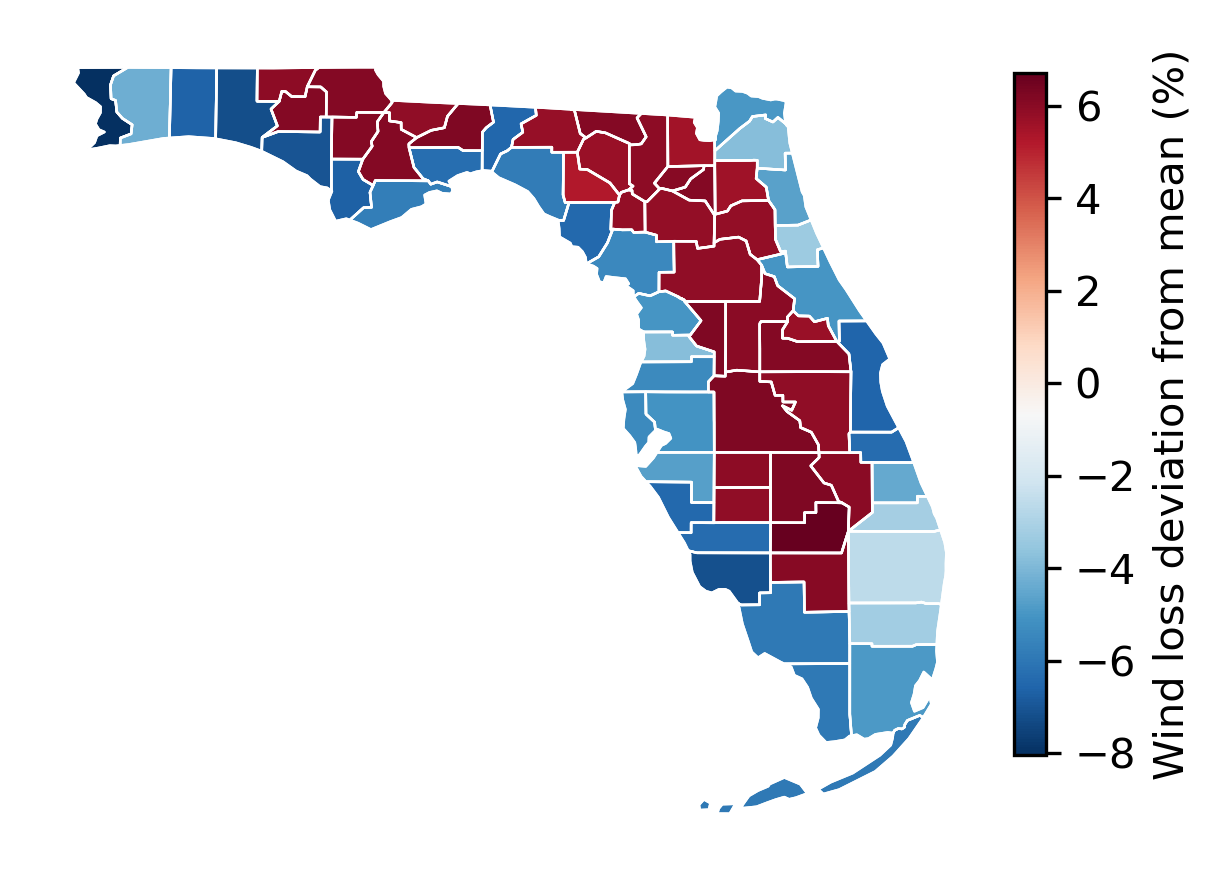
\includegraphics[width=0.45\textwidth]{figures/wind_loss_deviation.png}
    \caption{\textbf{County-level deviation in wind loss attribution across Florida.} 
    Percentage-point deviation of county-specific wind shares from the state-wide mean, derived from events at or above the county 95th percentile of compound hazard intensity in the synthetic tropical cyclone event set (Text~S2). Positive values indicate wind-dominated counties; negative values indicate relatively stronger flood contributions.}
\label{FigWindLossDeviation}
\end{figure*}

\begin{figure*}[htb!]
    \centering
    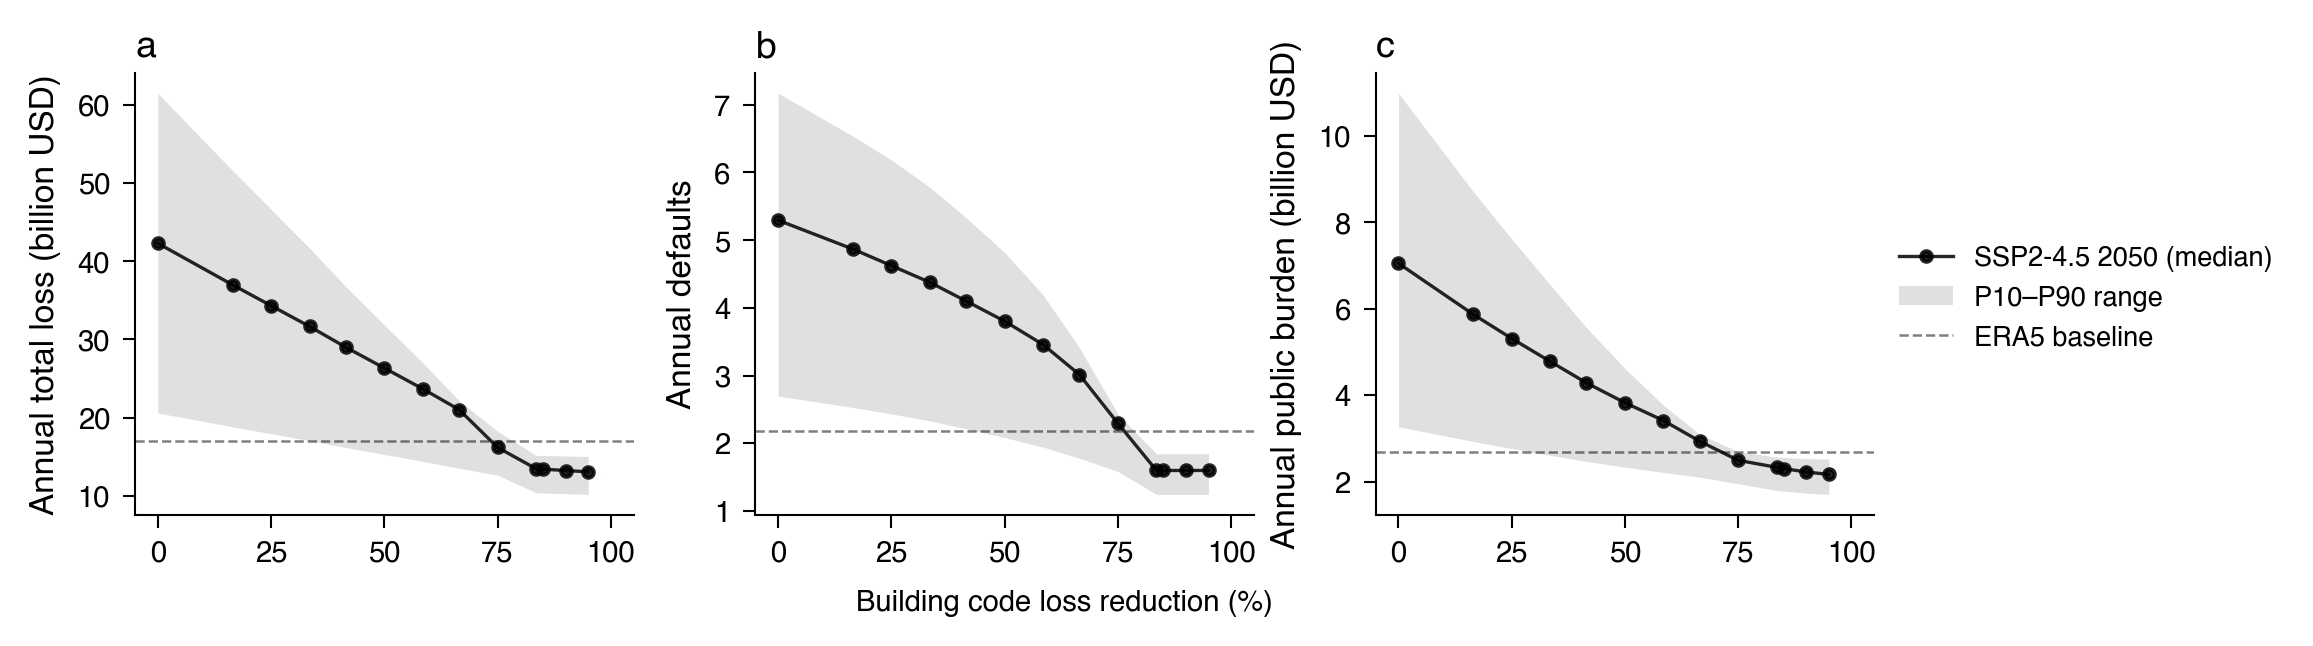
\includegraphics[width=1.0\textwidth]{figures/fig_climate_buildingcode_sensitivity.png}
    \caption{\textbf{Sensitivity of systemic insurance outcomes to prescribed loss reductions under future climate conditions.} Sensitivity analysis showing the effect of incremental reductions in wind- and flood-related losses representing the effects of stronger building standards and retrofitting on systemic risk outcomes under mid-century (2041-2060) SSP2-4.5 climate conditions. Shown are a) annual total loss, b) annual number of private insurer defaults, and c) annual total public burden. Solid lines indicate results for the median climate-induced risk change across the GCM ensemble, shaded bands show the 10th--90th percentile range across GCMs, and dashed lines denote the present-day ERA5 baseline. All quantities represent mean annual outcomes across \num{10000} simulated tropical cyclone seasons per climate realization.}
\label{FigClimateBuildingCodeSensitivity}
\end{figure*}

\clearpage
\renewcommand{\refname}{Supplementary References}
\bibliography{systemic_risk_fl}

\end{document}